\renewcommand{\baselinestretch}{1.2} 
\chapter{Bài 21. ĐỘNG LỰC HỌC CỦA CHUYỂN ĐỘNG TRÒN.\\ LỰC HƯỚNG TÂM}
\begin{center}
	\textit{(Tiết 1)}
\end{center}
\section{MỤC TIÊU DẠY HỌC}
\begin{center}
	\begin{longtable}{|M{2.5cm}|L{12.5cm}|M{2cm}|}
		\hline
		\thead{Biểu hiện\\ năng lực} & \thead{Mục tiêu} & \thead{STT}\\
		\hline
		\multicolumn{3}{|c|}{\textbf{ Năng lực vật lí}}\\
		\hline
		1.1 & Nêu được phương, chiều lực hướng tâm. & 1\\
		\hline
		1.1 & Nêu được điều kiện để vật chuyển động tròn đều. & 2\\
		\hline
		1.1 & Trình bày được vai trò của lực hướng tâm trong chuyển động tròn đều. & 3\\
		\hline
		3.1& Vận dụng được biểu thức lực hướng tâm $F=m\omega^2r$, $F=mv^2/r$. & 4\\
		\hline
		\multicolumn{3}{|c|}{\textbf{Năng lực chung}}\\
		\hline
		TC - TH& Tích cực thực hiện các nhiệm vụ GV đặt ra cho các nhóm, tích cực suy luận để đưa ra câu trả lời trong quá trình GV định hướng nội dung học tập	&5 \\
		\hline
		GT - HT& Xác định nhiệm vụ và hoạt động của bản thân - phân tích được các công việc cần thực hiện để hoàn thành nhiệm vụ của nhóm.	& 6 \\
		\hline
	\end{longtable}
\end{center}
\section{THIẾT BỊ DẠY HỌC VÀ HỌC LIỆU}
\begin{itemize}
	\item Tivi/máy chiếu;
	\item SGK;
	\item Dụng cụ thí nghiệm đơn giản.
\end{itemize}
\section{TIẾN TRÌNH DẠY HỌC}
\subsection{TIẾN TRÌNH}
\begin{center}
	\begin{longtable}{|L{2.75cm}|C{1.25cm}|L{5cm}|L{3.5cm}|L{4cm}|}
		\hline
		\thead{Tiến trình} & \thead{Mục\\tiêu} & \thead{Nội dung dạy học \\trọng tâm} & \thead{PP,\\ KTDH} & \thead{Phương pháp \\đánh giá}\\
		\hline
		\textbf{Hoạt động 1:} Nhắc lại kiến thức động học của chuyển động tròn đều&5  & \begin{itemize}
			\item Gia tốc và vận tốc trong chuyển động tròn đều.
			\item Mối liên hệ giữa gia tốc và lực (Định luật II Newton).
		\end{itemize} &PPDH: Đàm thoại  &GV đánh giá dựa trên câu trả lời của HS.\newline
		PP đánh giá: quan sát, nghe.  \\
		\hline
		\textbf{Hoạt động 2:} Tìm hiểu lực hướng tâm & 1, 2, 5& Đặc điểm và biểu thức lực hướng tâm. &PPDH: Đàm thoại  &GV đánh giá dựa trên câu trả lời của HS.\newline PP đánh giá: quan sát, nghe.  \\
		\hline
		\textbf{Hoạt động 3:} Lực hướng tâm không phải là loại lực mới & 3, 4, 6& Lực hướng tâm là lực hoặc hợp lực của các lực đã học. &PPDH: Dạy học hợp tác  &GV đánh giá dựa trên câu trả lời của HS và kết quả hoạt động nhóm.\newline PP đánh giá: quan sát, nghe.  \\
		\hline
		\textbf{Hoạt động 4:} Bài toán xác định tốc độ tối thiểu để vật chuyển động trên quỹ đạo tròn & 4, 6& Vận dụng biểu thức lực hướng tâm $F=mv^2/r$. &PPDH: Dạy học hợp tác  &GV đánh giá dựa trên câu trả lời của HS và kết quả hoạt động nhóm.\newline PP đánh giá: quan sát, nghe.  \\
		\hline
	\end{longtable}
\end{center}
\subsection{CÁC HOẠT ĐỘNG HỌC}
\hoatdong{Nhắc lại kiến thức động học của chuyển động tròn đều}
{
\begin{itemize}
	\item HS nêu được biểu thức xác định tốc độ dài và gia tốc hướng tâm.
	\item HS xác định được phương, chiều của vector vận tốc và vector gia tốc của vật chuyển động tròn đều.
	\end{itemize}}
{Câu trả lời của HS.
}
{\textit{\underline{* GV chuyển giao nhiệm vụ học tập}}\\
	\begin{itemize}[label=$-$]
		\item GV yêu cầu HS xác định hướng vector vận tốc và vector gia tốc tại một điểm trên bánh xe đang quay.
		\begin{center}
	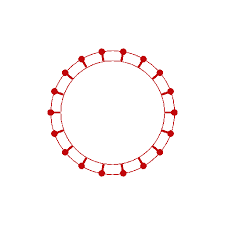
\includegraphics[scale=0.6]{figs/G10-BAI21-1}
		\end{center}
		\item GV yêu cầu HS viết biểu thức xác định độ lớn vận tốc và gia tốc hướng tâm của vật chuyển động tròn.
		\item GV đặt câu hỏi gợi mở để ôn lại định luật II Newton:
		\begin{itemize}[label=$\bullet$]
			\item Nếu có một chiếc xe bị tắt máy trên đường, làm thế nào để xe này có thể tăng tốc (thu gia tốc)?
			\begin{center}
				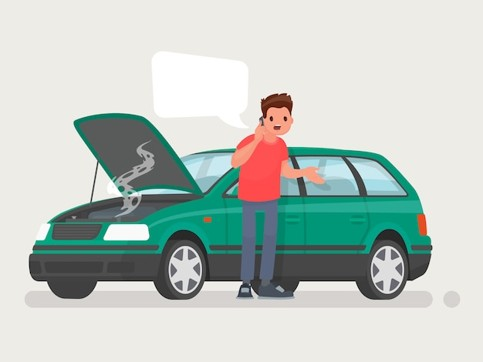
\includegraphics[scale=0.5]{figs/G10-BAI21-2}
			\end{center}
			\item Để vật chuyển động có gia tốc thì phải có lực hoặc hợp lực tác dụng lên vật, gia tốc và lực có mối liên hệ với nhau như thế nào?
		\end{itemize}
	\end{itemize}
	\textit{\underline{* HS thực hiện nhiệm vụ học tập}}\\
	HS lần lượt trả lời câu hỏi của GV:
	\begin{itemize}
		\item Vector vận tốc tiếp tuyến quỹ đạo và cùng hướng chuyển động, vector gia tốc hướng vào tâm quỹ đạo.
		\item Độ lớn vận tốc và gia tốc hướng tâm: $v=\omega R$; $a_{\mathrm{ht}}=\omega^2R=\dfrac{v^2}{R}$.
		\item Để xe thu gia tốc thì người ta phải tác dụng lực kéo/đẩy lên xe.
		\item Định luật II Newton: $\vec{F}=m\vec{a}$.
			\end{itemize}
			\textit{\underline{* HS báo cáo kết quả nhiệm vụ học tập}}\\
			HS giơ tay phát biểu, GV mời 1 em HS trả lời 1 câu hỏi.
}
\hoatdong{Tìm hiểu lực hướng tâm}
{\begin{itemize}
		\item HS nêu được phương, chiều của lực hướng tâm.
		\item HS nêu được điều kiện để vật chuyển động tròn đều.
		\item HS vận dụng được biểu thức lực hướng tâm $F=m\omega^2 R$, $F=mv^2/R$.
	\end{itemize}
}
{Phần trả lời của HS về đặc điểm và biểu thức tính độ lớn của lực hướng tâm.

}
{\textit{\underline{* GV chuyển giao nhiệm vụ học tập}}\\
	GV lần lượt đặt câu hỏi gợi mở để hướng dẫn HS tìm hiểu về đặc điểm của lực hướng tâm:
	\begin{itemize}[label=$-$]
		\item Trong quá trình vật chuyển động tròn đều, gia tốc của vật luôn hướng vào tâm quỹ đạo. Từ định luật II Newton ta thiết lập được mối liên hệ giữa lực và gia tốc hướng tâm:
		$$\vec{F}_{\mathrm{ht}}=m\vec{a}_{\mathrm{ht}}.$$
		\item Từ mối liên hệ lực và gia tốc trong định luật II Newton, em hình cho biết phương chiều của lực hướng tâm.
		\item Từ biểu thức tính độ lớn của gia tốc hướng tâm, em hãy suy ra biểu thức xác định độ lớn của lực hướng tâm.
		\item GV yêu cầu HS thực hiện \textbf{Bài tập 1} theo hình thức cá nhân.
	\end{itemize}
		\textit{\underline{* HS thực hiện nhiệm vụ học tập}}\\
	HS lần lượt trả lời câu hỏi của GV:
	\begin{itemize}
		\item Vector lực hướng tâm cùng hướng với vector gia tốc hướng tâm. Như vậy lực hướng tâm có:
		\begin{itemize}
			\item Phương: trùng phương bán kính.
			\item Chiều: hướng vào tâm quỹ đạo.
		\end{itemize}
		\item Từ biểu thức xác định độ lớn gia tốc hướng tâm $a_{\mathrm{ht}}=\omega^2R=\dfrac{v^2}{R}\Rightarrow F_{\mathrm{ht}}=m\omega^2 R=m\dfrac{v^2}{R}$.
	\end{itemize}
	HS thực hiện \textbf{Bài tập 1} theo hình thức cá nhân.\\
\textit{\underline{* HS báo cáo kết quả nhiệm vụ học tập}}\\
HS giơ tay phát biểu, GV mời 1 em HS trả lời 1 câu hỏi.\\
HS xung phong lên bảng trình bày kết quả \textbf{Bài tập 1}, GV mời 1 HS bất kì nhận xét bài làm của bạn.
}
\hoatdong{Lực hướng tâm không phải là loại lực mới}
{\begin{itemize}
		\item HS trình bày được vai trò của lực hướng tâm trong chuyển động tròn đều.
		\item HS vận dụng được biểu thức lực hướng tâm $F=m\omega^2 R$, $F=mv^2/R$.
	\end{itemize}

}
{Câu trả lời của HS cho các câu hỏi gợi mở của GV.\\
	Kết quả bài tập nhóm.

}
{\textit{\underline{* GV chuyển giao nhiệm vụ học tập}}\\
	GV dẫn dắt HS xác định lực nào đóng vai trò lực hướng tâm lần lượt trong 4 ví dụ:
	\begin{itemize}
		\item \textbf{Ví dụ 1:} Quay vật nhẹ trong mặt phẳng song song với mặt đất.
		\begin{itemize}
			\item GV đặt câu hỏi: Nếu dây bị đứt trong quá trình quay thì vật sẽ chuyển động như thế nào?
			\item Từ đó em hãy cho biết vai trò của lực hướng tâm trong chuyển động tròn.
		\end{itemize}
		\item \textbf{Ví dụ 2:} Chuyển động của Mặt Trăng quanh Trái Đất.
		\begin{center}
			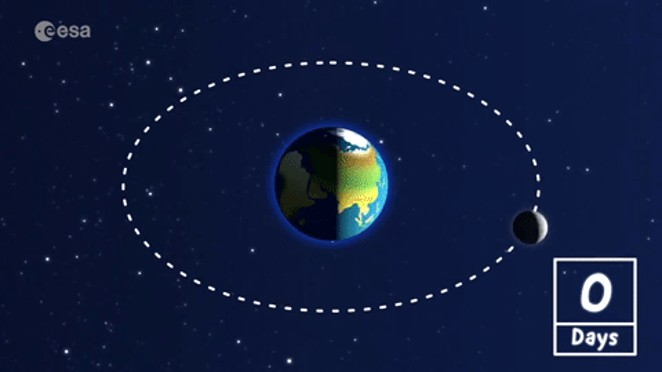
\includegraphics[scale=0.5]{figs/G10-BAI21-3}
		\end{center}
		\begin{itemize}
			\item GV đặt câu hỏi: Trong trường hợp này không có sợi dây nào nối Mặt Trăng và Trái Đất, vậy tại sao Mặt Trăng của thể chuyển động tròn xung quanh Mặt Trăng?
			\item GV yêu cầu HS thảo luận nhóm đôi để thực hiện \textbf{Bài tập 2}.
		\end{itemize}
		\item \textbf{Ví dụ 3:} GV đặt tình huống có vấn đề: Làm thế nào để một tờ giấy A4 có thể cắt qua được miếng mút xốp.
		\begin{center}
			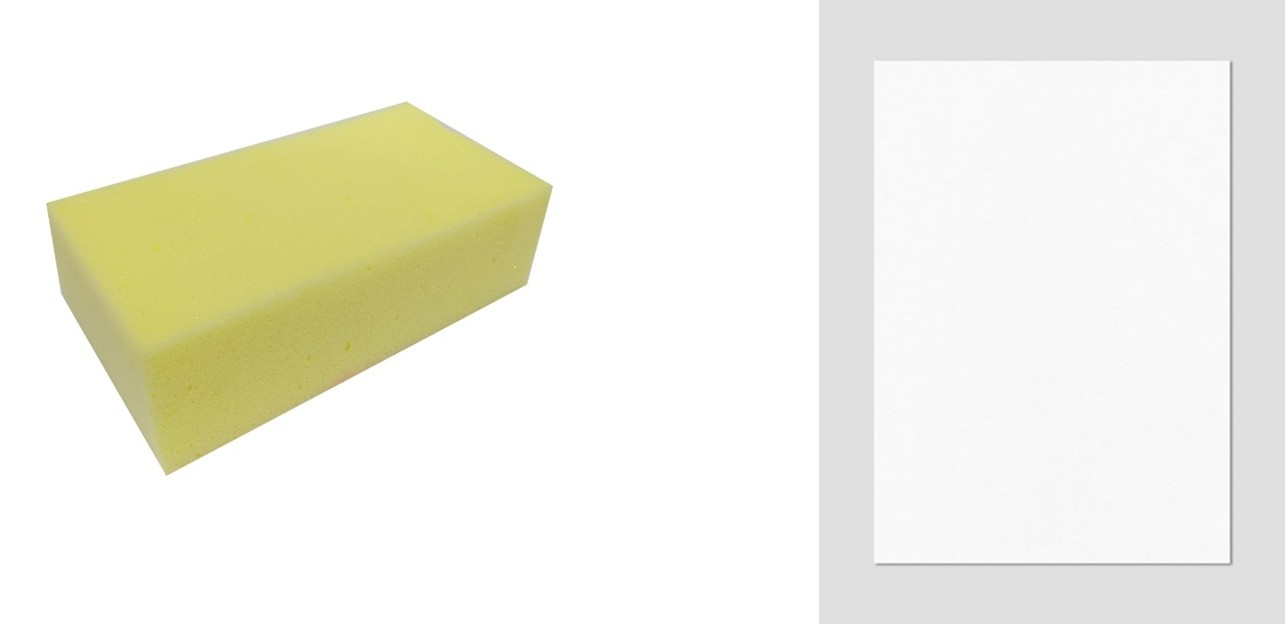
\includegraphics[scale=0.5]{figs/G10-BAI21-4}
		\end{center}
		HS suy nghĩ và xung phong lên bảng để thử thực hiện.\\
		GV mời lần lượt 2 - 3 em HS lên bảng để thử nghiệm.\\
		GV tiến hành thực hiện cho HS xem:
		\begin{itemize}
			\item \textbf{\textit{Cách 1:}} Cố gắng đè chặt miếng xốp rồi dùng giấy cắt mạnh qua, hoặc gấp giấy lại thành nhiều lớp vẫn không cắt qua được.
			\item \textbf{\textit{Cách 2:}} Cắt giấy A4 thành hình tròn đường kính \SI{6}{\centi\meter}, gắn mảnh giấy tròn vào đầu máy khoan. Bật cho máy khoan quay, mảnh giấy dễ dàng cắt qua miếng xốp.
			\begin{center}
				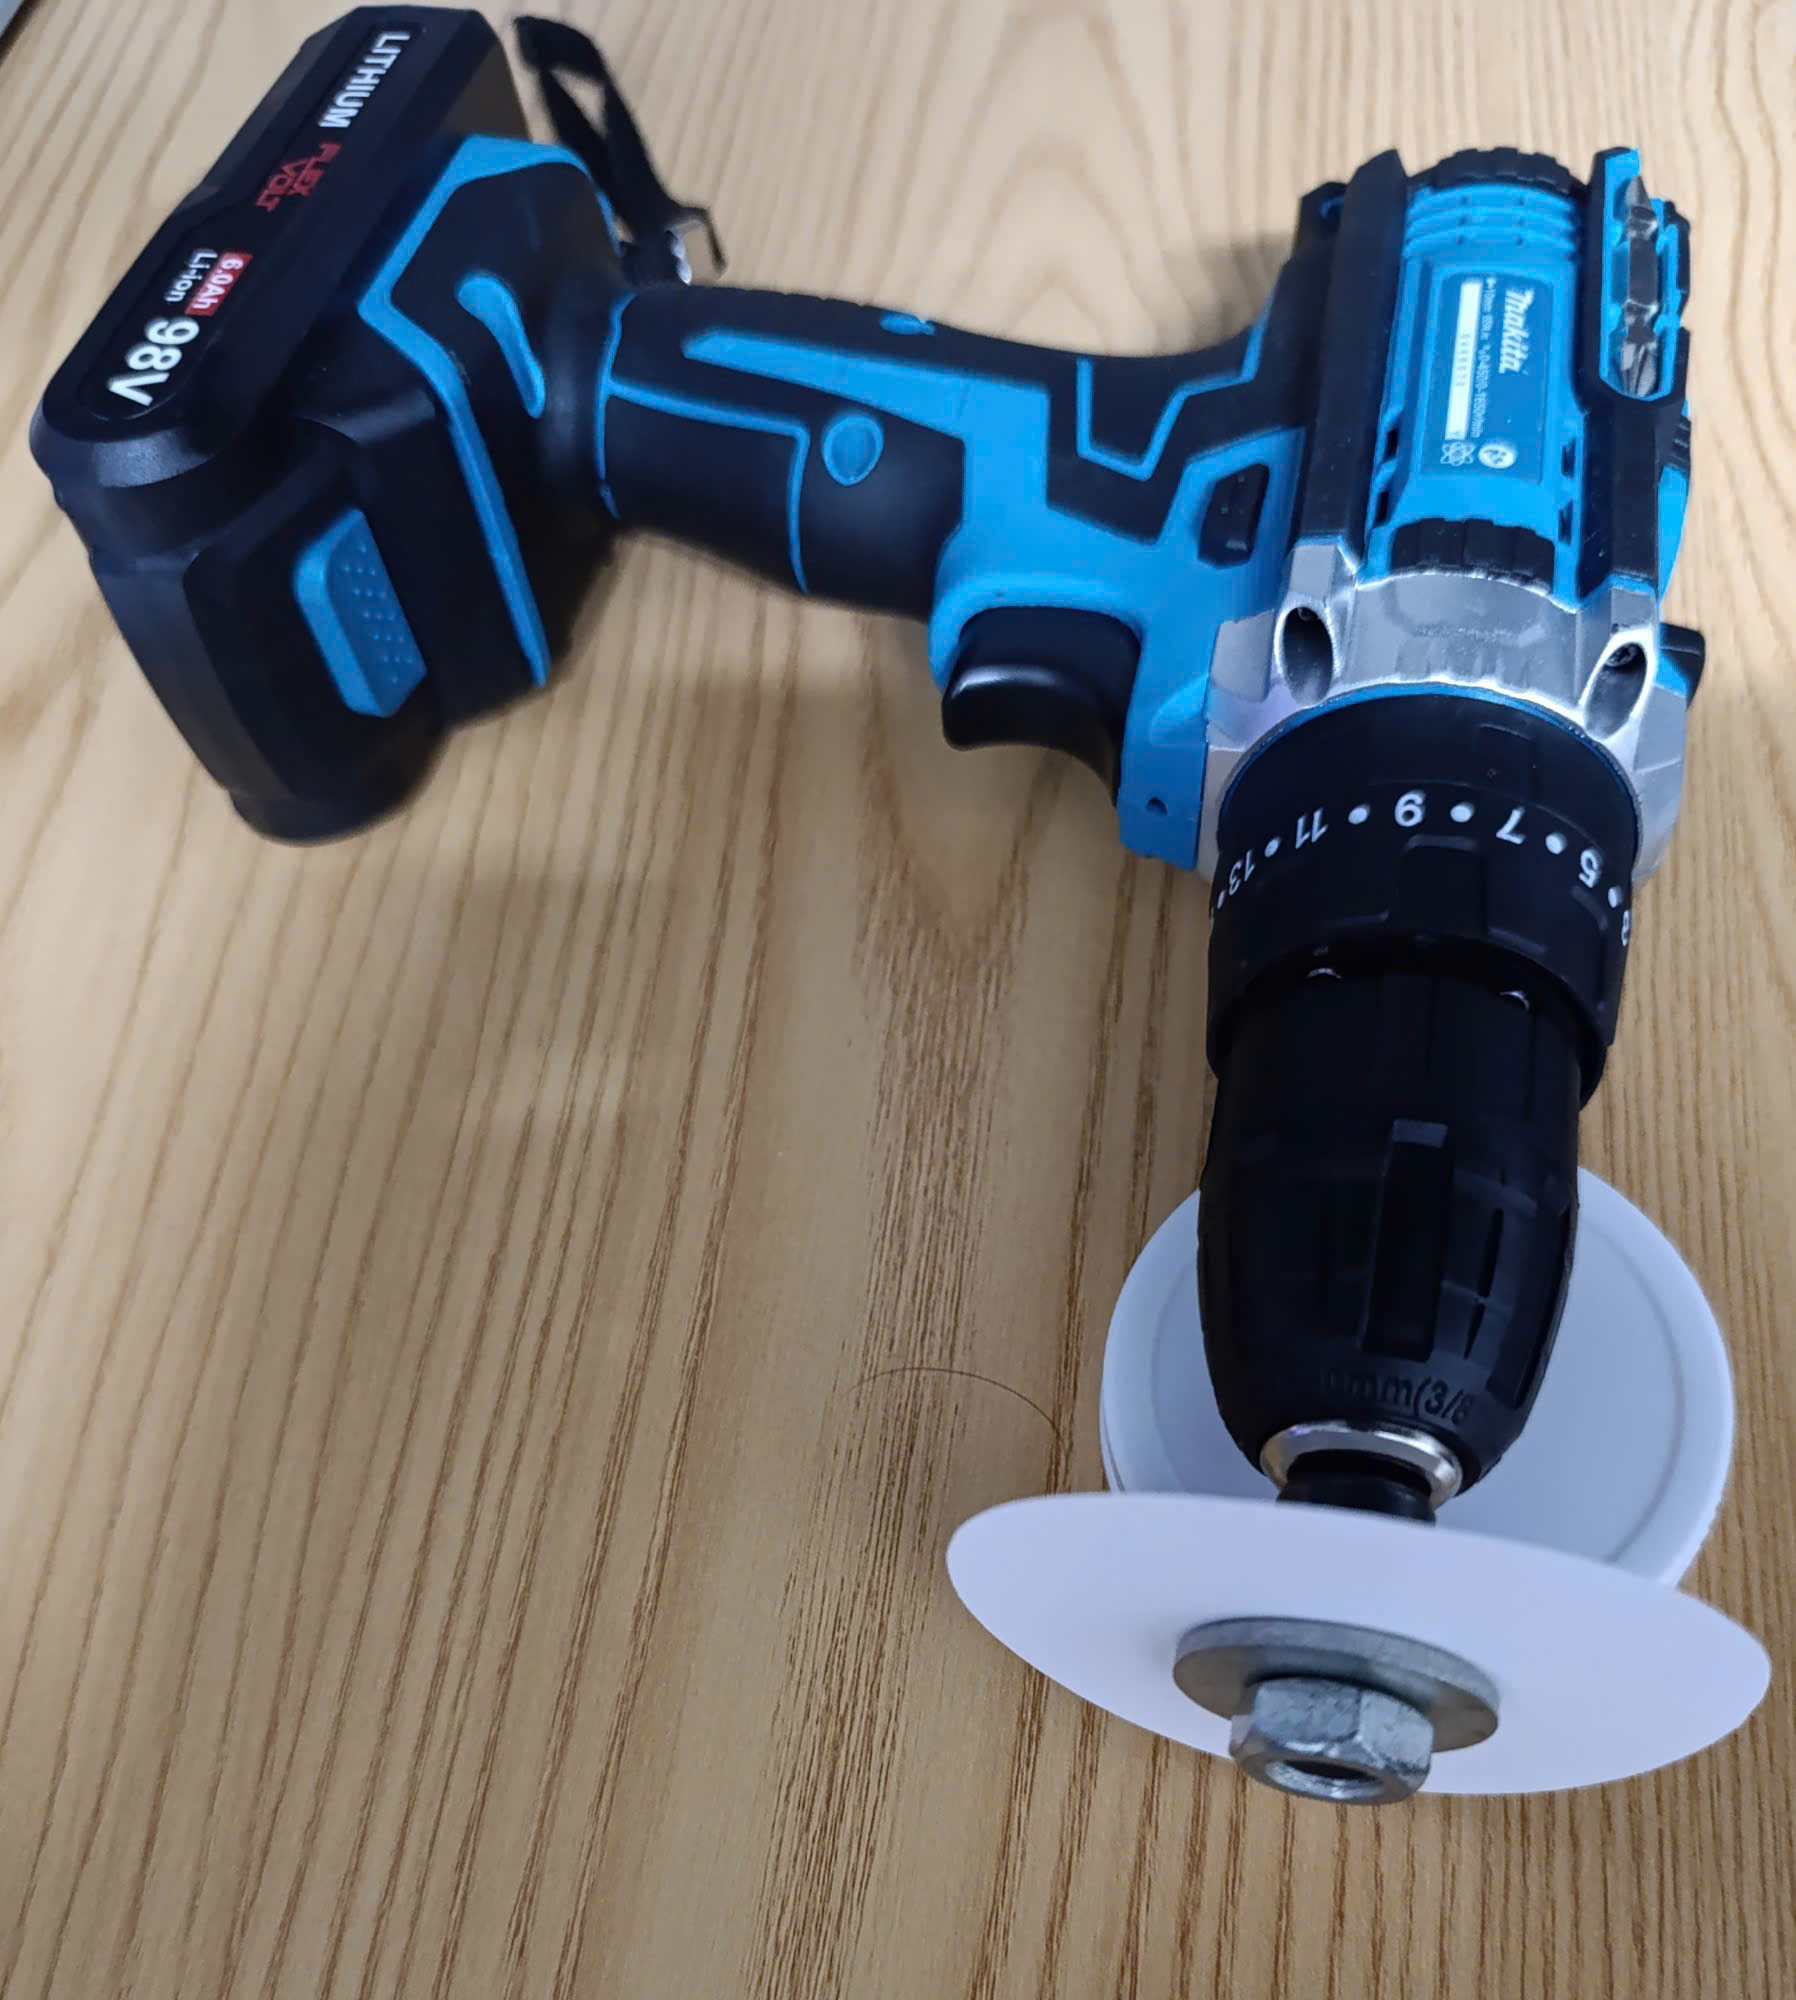
\includegraphics[scale=0.1]{figs/G10-BAI21-5}
			\end{center}
		\end{itemize}
		GV đặt câu hỏi: Vì sao khi cho mảnh giấy quay tròn thì nó có thể dễ dàng cắt qua được mút xốp?\\
		Trường hợp HS không trả lời được, GV làm thêm thí nghiệm phụ:
		\begin{itemize}
			\item Cắt đáy chai nước suối \SI{500}{\milli\liter}, gắn chai nước vào đầu mũi khoan.
			\item Tròng dây xích qua thân chai nhựa. Cho máy khoan quay, từ từ đẩy dây xích ra khỏi vỏ chai, dây xích tiếp tục lăn tròn vài vòng trên mặt phẳng nằm ngang trước khi dừng lại.
			\begin{center}
				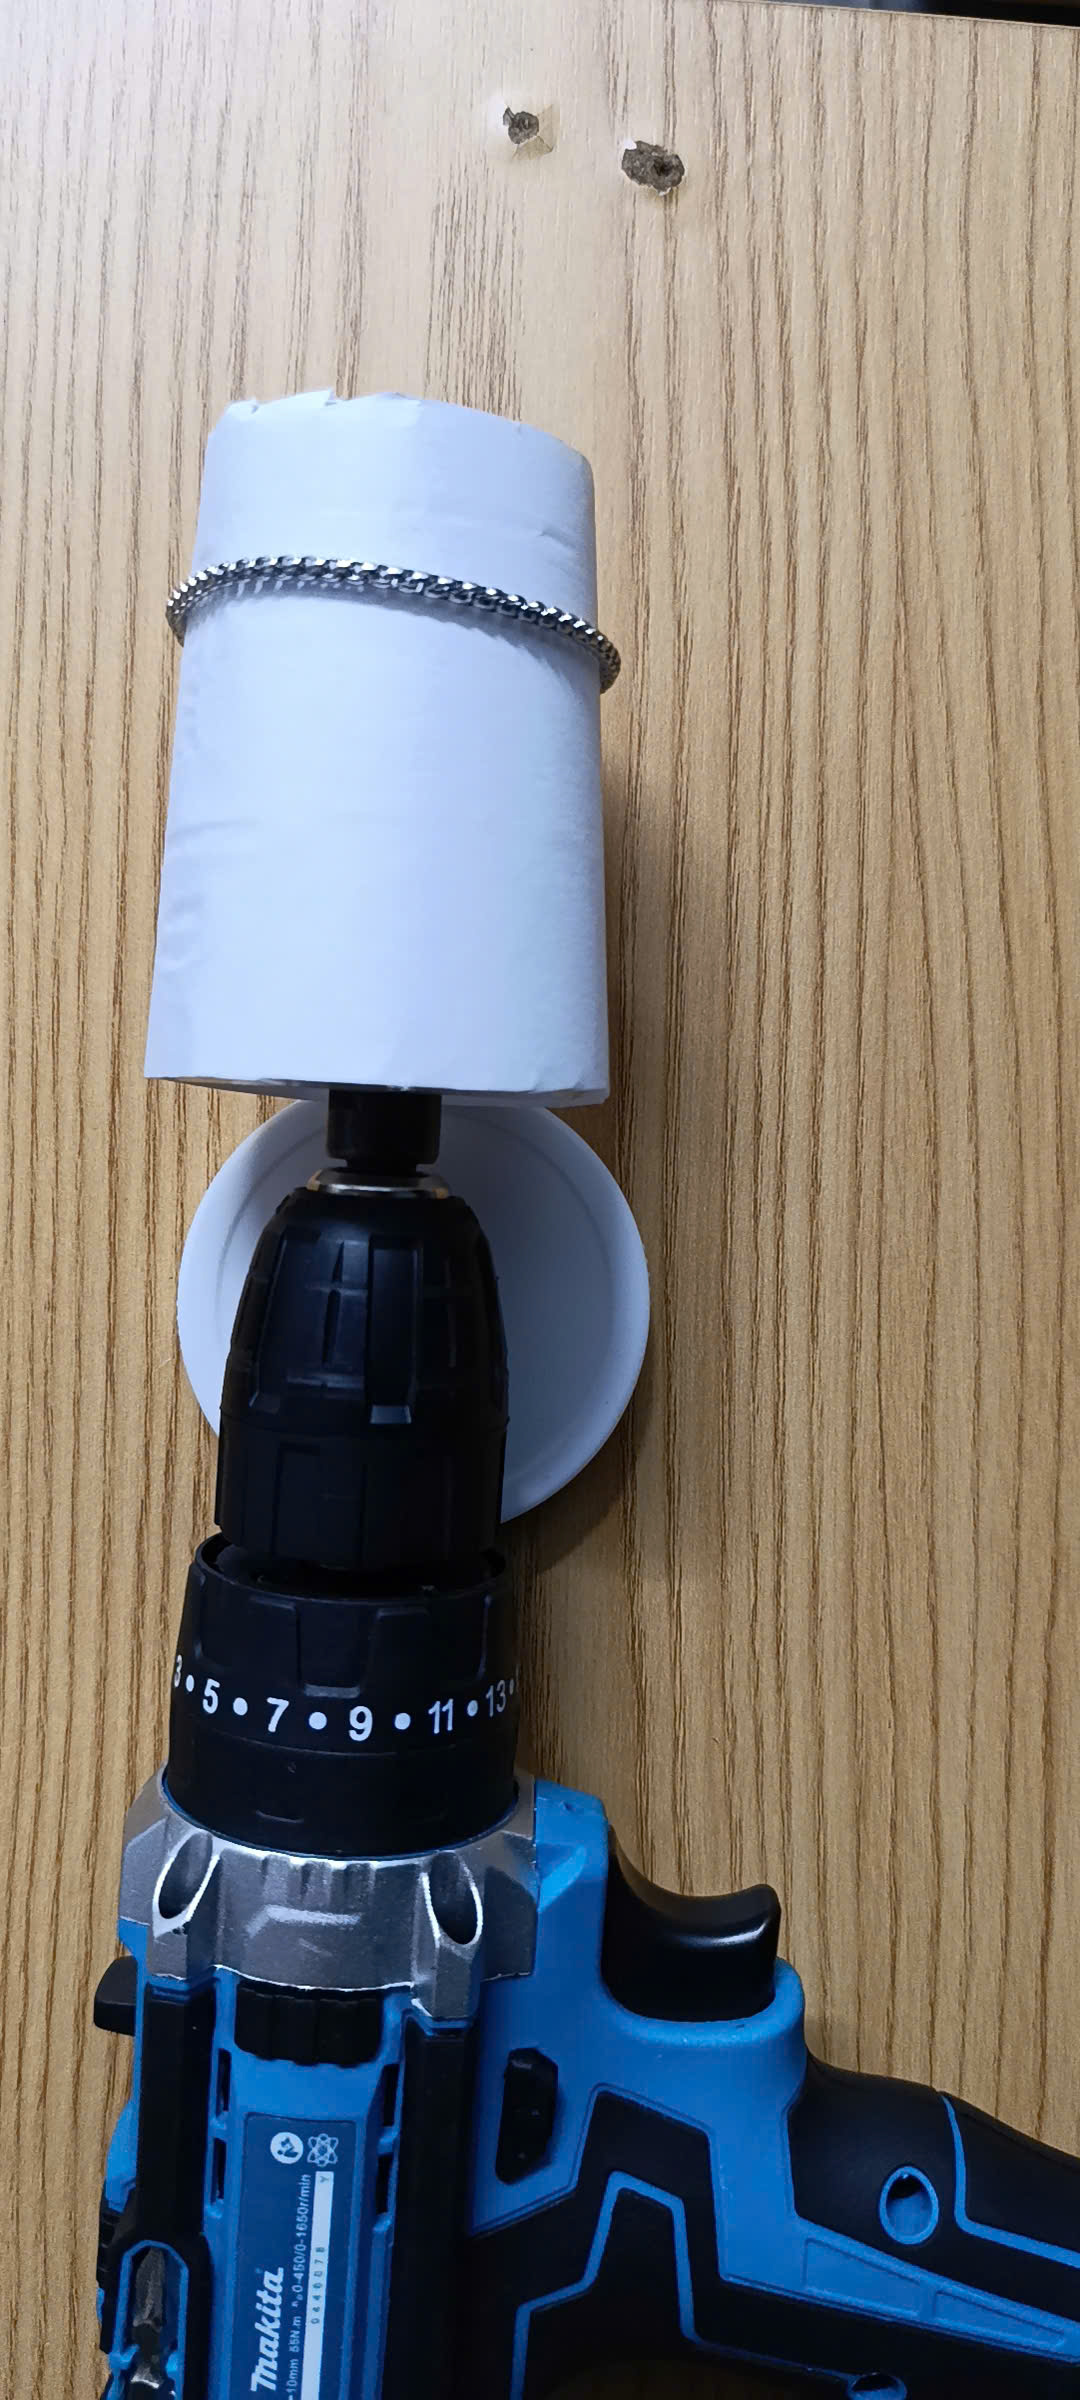
\includegraphics[scale=0.1, angle=-90]{figs/G10-BAI21-6}
			\end{center}
		\end{itemize}
		GV đặt câu hỏi: Vì sao ban đầu dây xích rất "mềm" không thể giữ được dạng vòng tròn, nhưng khi quay lại có thể chuyển động tròn trên mặt bàn?
		\item \textbf{Ví dụ 4:} GV đặt tình huống có vấn đề: GV đặt một cốc nước lên bàn và yêu cầu HS tìm cách lật ngược cốc nước lại nhưng nước không đổ ra ngoài.
		\begin{center}
			
\includegraphics[scale=0.4]{figs/G10-BAI21-7}
		\end{center}
		GV thực hiện thí nghiệm để HS xem.
		\begin{center}
			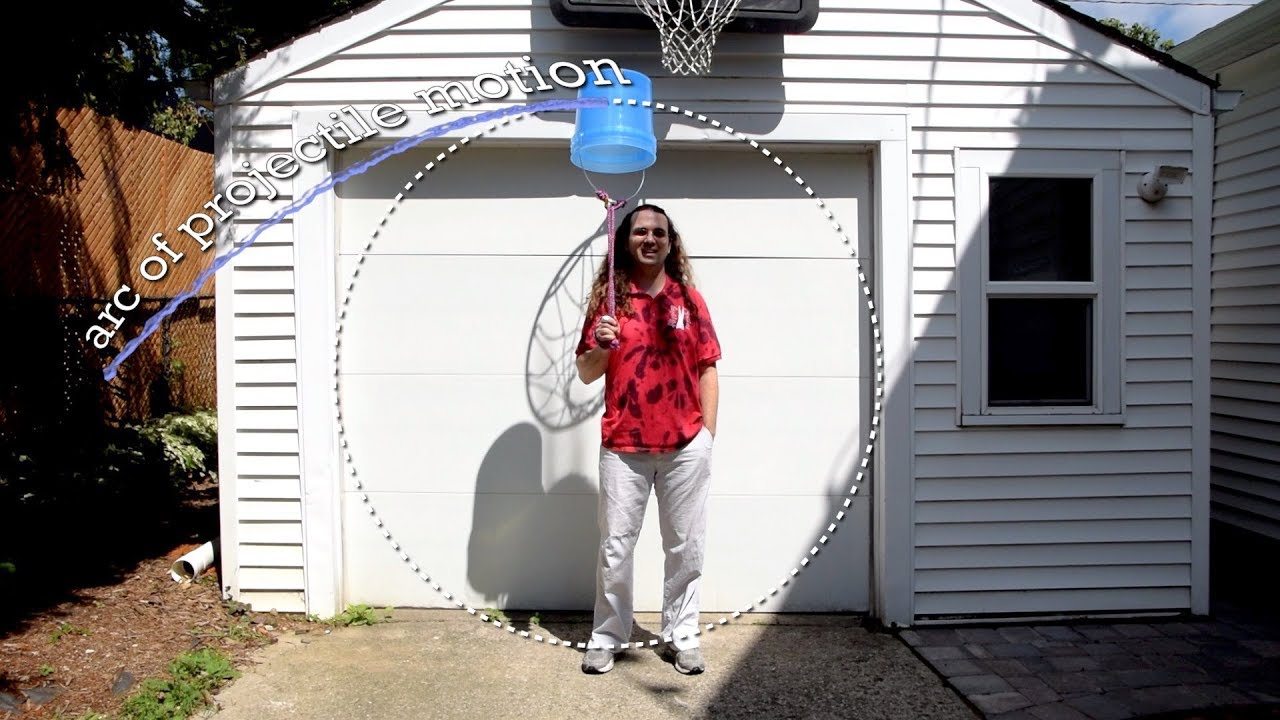
\includegraphics[scale=0.25]{figs/G10-BAI21-9}
		\end{center}
		GV yêu cầu HS xác định các lực tác dụng lên khối nước khi cốc chuyển động lên đến vị trí cao nhất.\\
		GV yêu cầu HS xác định lực đóng vai trò là lực hướng tâm tác dụng lên khối nước khi ở vị trí cao nhất.
			\end{itemize}
			Sau 4 ví dụ, GV mời HS nhận xét về bản chất của lực hướng tâm: Lực hướng tâm có phải là loại lực mới không? Vậy lực hướng tâm có bản chất là lực gì?\\
\textit{\underline{* HS thực hiện nhiệm vụ học tập}}\\
HS suy nghĩ và trả lời câu hỏi của GV qua từng ví dụ:
\begin{itemize}
	\item \textbf{Ví dụ 1:}
	\begin{itemize}
		\item Nếu dây bị đứt, vật sẽ văng ra theo phương vuông góc với sợi dây (tiếp tuyến quỹ đạo).
		\item Lực hướng tâm trong ví dụ 1 là lực căng dây. Vậy lực hướng tâm có vai trò giữ cho vật chuyển động trên quỹ đạo tròn.
	\end{itemize}
	\item \textbf{Ví dụ 2:}
	\begin{itemize}
		\item Lực hấp dẫn của Trái Đất tác dụng lên Mặt Trăng đóng vai trò là lực hướng tâm làm cho Mặt Trăng chuyển động tròn xung quanh Trái Đất.
		\item HS hoạt động nhóm đôi để thực hiện Bài tập 2.
	\end{itemize}
	\item \textbf{Ví dụ 3:} 
	\begin{itemize}
		\item HS xung phong lên bảng để thử cắt miếng mút xốp bằng giấy A4.
		\item Dự đoán câu trả lời của HS cho câu hỏi phụ: Các mắc xích được liên kết với nhau, ở trạng thái ban đầu dây xích không bị kéo căng, do đó lực liên kết giữa các mắc bằng 0. Khi cho dây xích quay tròn, các mắc xích được kéo căng nhờ lực căng của hai phần tử bên cạnh. Hợp lực kéo của hai phần tử bên cạnh đóng vai trò là lực hướng tâm giữ cho mắc xích chuyển động tròn. Khi quay với tốc độ càng cao, độ lớn lực hướng tâm càng lớn, do đó lực kéo của hai phần tử bên cạnh càng tăng, xích càng "cứng".\\
		Tương tự, HS giải thích cho chuyển động của miếng giấy A4 khi gắn vào mũi khoan.
		\begin{center}
			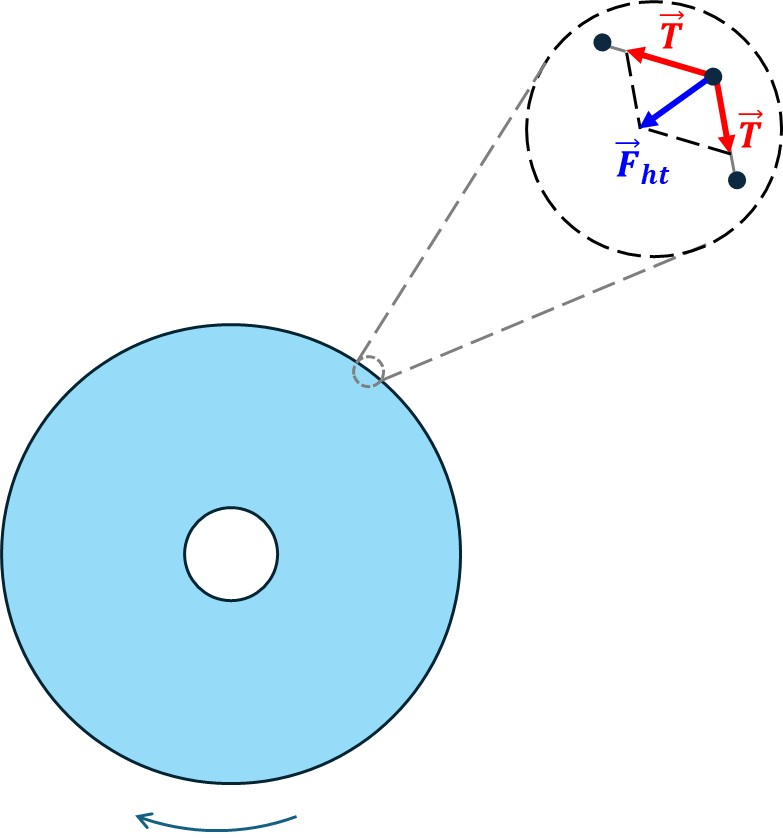
\includegraphics[scale=0.4]{figs/G10-BAI21-8}
		\end{center}
	\end{itemize}
	\item \textbf{Ví dụ 4:}
	\begin{itemize}
		\item HS trình bày hướng giải quyết vấn đề của mình bằng cách giơ tay phát biểu.
		\item HS xác định lực tác dụng vào khối nước tại vị trí cao nhất: Trọng lực và phản lực do đáy lọ tác dụng lên khối nước.
		\item HS xác định lực hướng tâm tác dụng lên khối nước ở vị trí cao nhất: Hợp lực của trọng lực và phản lực
		$$P+N=ma_{\mathrm{ht}}.$$
	\end{itemize}
	HS trình bày suy nghĩ về bản chất của lực hướng tâm sau 4 ví dụ.
\end{itemize}
\textit{\underline{* HS báo cáo kết quả nhiệm vụ học tập}}
\begin{itemize}
	\item HS xung phong trả lời các câu hỏi.
	\item GV chuẩn hóa kiến thức: Lực hướng tâm không phải là loại lực mới. Lực hướng tâm là lực hoặc hợp lực của các lực đã học (lực hấp dẫn, lực căng dây, lực ma sát, \dots)
	\item GV giới thiệu ứng dụng của ví dụ 3 và 4 trong thực tế:
	\begin{itemize}
		\item Ví dụ 3: Ứng dụng chuyển động tròn trong máy cắt.
		\begin{center}
			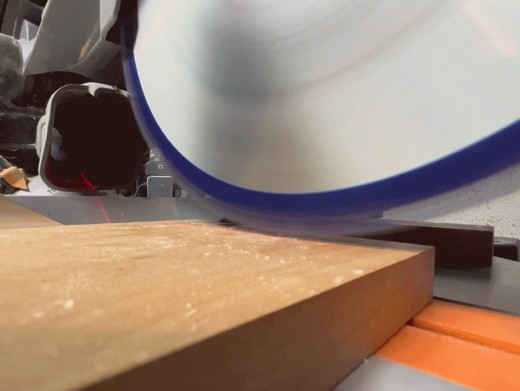
\includegraphics[scale=0.4]{figs/G10-BAI21-10}
		\end{center}
		\item Ví dụ 4: Tàu lượn siêu tốc.
		\begin{center}
			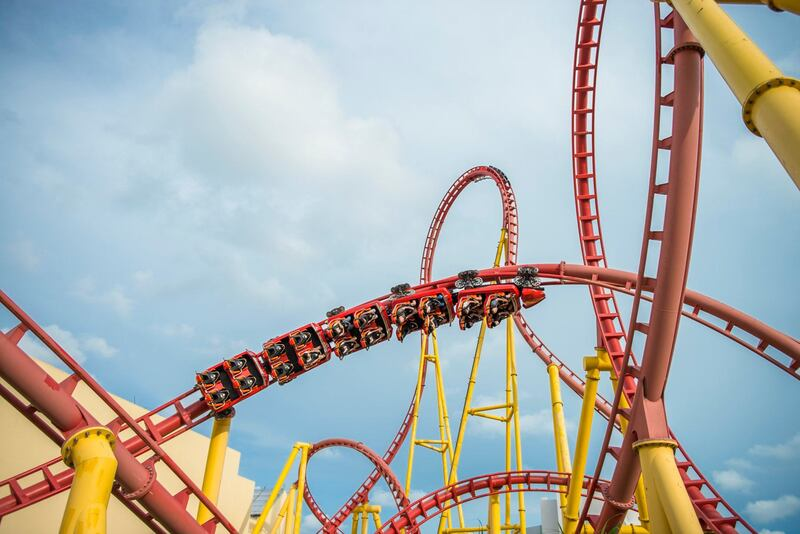
\includegraphics[scale=0.25]{figs/G10-BAI21-11}
		\end{center}
	\end{itemize}
\end{itemize}
}
\hoatdong{Bài toán xác định tốc độ tối thiểu để vật chuyển động trên quỹ đạo tròn}
{HS vận dụng được biểu thức xác định lực hướng tâm $F=mv^2/r$}
{Kết quả thảo luận nhóm của nhóm HS.
}
{\textit{\underline{* GV chuyển giao nhiệm vụ học tập}}\\
	GV đặt câu hỏi mở đầu: Trong ví dụ 4, khi quay càng nhanh hay quay càng chậm thì nước sẽ khó rơi ra ngoài hơn?\\
	Vậy bây giờ chúng ta hãy thử xác định tốc độ quay tối thiểu để nước không rơi ra ngoài.\\
	GV yêu cầu HS thảo luận với nhóm 4 HS và thực hiện \textbf{Bài tập 3}.\\
	\textit{\underline{* HS thực hiện nhiệm vụ học tập}}\\
	HS thảo luận theo nhóm.\\
	GV hỗ trợ các nhóm HS khi gặp vấn đề khó khăn.\\
	\textit{\underline{* HS báo cáo kết quả nhiệm vụ học tập}}\\
	GV mời đại diện nhóm HS có kết quả sớm nhất lên trình bày kết quả bài tập và giải thích hướng giải quyết vấn đề.\\
	GV mời 1 HS bất kì nhận xét kết quả của nhóm bạn.\\
	GV chỉnh lý, hợp thức hóa kiến thức.

}
\section{CÁC HỒ SƠ KHÁC}
\subsection{NỘI DUNG DẠY HỌC}
\begin{enumerate}[label=\bfseries\Roman*.]
	\item \textbf{LỰC HƯỚNG TÂM}\\
	Lực hướng tâm $\vec{F}_{\mathrm{ht}}$ có:
	\begin{itemize}
		\item phương: dọc theo bán kính;
		\item chiều: hướng vào tâm quỹ đạo;
		\item độ lớn:
		$$F_{\mathrm{ht}}=m\cdot a_{\mathrm{ht}}=m\cdot\dfrac{v^2}{R}=m\cdot\omega^2\cdot R.$$
	\end{itemize}
	Trong đó:
	\begin{itemize}
		\item $F_{\mathrm{ht}}$: lực hướng tâm $\left(\si{\newton}\right)$;
		\item $m$: khối lượng của vật $\left(\si{\kilogram}\right)$;
		\item $a_{\mathrm{ht}}$: gia tốc hướng tâm $\left(\si{\meter/\second^2}\right)$;
		\item $v$: tốc độ dài $\left(\si{\meter/\second}\right)$;
		\item $\omega$: tốc độ góc $\left(\si{\radian/\second}\right)$;
		\item $R$: bán kính quỹ đạo $\left(\si{\meter}\right)$.
	\end{itemize}
	\item \textbf{ỨNG DỤNG THỰC TẾ CỦA CHUYỂN ĐỘNG TRÒN}\\
	\textbf{Ví dụ 1:} Chuyển động của vật buộc bởi dây quay đều trong mặt phẳng nằm ngang.\\
	Lực căng dây đóng vai trò là lực hướng tâm.\\
	\textbf{Ví dụ 2:} Chuyển động của Mặt Trăng quanh Trái Đất.\\
	Lực hấp dẫn đóng vai trò là lực hướng tâm.\\
	\textbf{Ví dụ 3:} Chuyển động của lưỡi cưa tròn.\\
 Hợp lực liên kết giữa các phân tử đóng vai trò là lực hướng tâm.\\
 \textbf{Ví dụ 4:} Chuyển động của tàu lượn siêu tốc.\\
 Hợp lực của trọng lực và phản lực do đường ray tác dụng đóng vai trò là lực hướng tâm.\\
 \textbf{Nhận xét:} Lực hướng tâm không phải là một loại lực mới, lực hướng tâm là một trong các lực đã học (lực hấp dẫn, lực căng dây, lực ma sát, \dots) hoặc hợp lực của các lực đó.
\end{enumerate}
\subsection{BÀI TẬP VÍ DỤ}
\renewtheorem{ex}{\color{blue}Bài tập}
\setcounter{ex}{0}
% ===============================================================
\begin{ex}
	\immini{Một chiếc xe đua có khối lượng \SI{800}{\kilogram} đi qua đoạn đường cong có bán kính $R=\SI{4.0E2}{\meter}$ với tốc độ \SI{50}{\meter/\second}. Xác định độ lớn lực hướng tâm tác dụng lên xe.
	}{
\includegraphics[scale=0.4]{figs/G10-BAI21-12}}
	\loigiai{
		
	}
\end{ex}
% ===============================================================
\begin{ex}
	Khoảng cách từ Mặt Trăng đến tâm Trái Đất là \SI{384400}{\kilo\meter}, khối lượng của Mặt Trăng là \SI{73.48E21}{\kilogram}, Mặt Trăng quay hết 1 vòng quanh Trái Đất mất 29 ngày. Coi chuyển động của Mặt Trăng quanh Trái Đất là chuyển động tròn đều.	\loigiai{
		
	}
\end{ex}
% ===============================================================
\begin{ex}
	Khoảng cách từ tâm khối nước đến tâm quỹ đạo là \SI{1}{\meter}. Gia tốc trọng trường $g=\SI{9.8}{\meter/\second^2}$. Tìm tốc độ tối thiểu ở vị trí cao nhất để nước không rơi ra khỏi lọ.
	\loigiai{
		
	}
\end{ex}
\begin{center}
	\textbf{--- HẾT ---}
\end{center}